\documentclass[11pt, a4paper, leqno]{article}
\usepackage{a4wide}
\usepackage[T1]{fontenc}
\usepackage[utf8]{inputenc}
\usepackage{float, afterpage, rotating, graphicx}
\usepackage{epstopdf}
\usepackage{longtable, booktabs, tabularx}
\usepackage{fancyvrb, moreverb, relsize}
\usepackage{eurosym, calc}
% \usepackage{chngcntr}
\usepackage{amsmath, amssymb, amsfonts, amsthm, bm}
\usepackage{caption}
\usepackage{mdwlist}
\usepackage{xfrac}
\usepackage{setspace}
\usepackage{xcolor}
\usepackage{subcaption}
\usepackage{minibox}
% \usepackage{pdf14} % Enable for Manuscriptcentral -- can't handle pdf 1.5
% \usepackage{endfloat} % Enable to move tables / figures to the end. Useful for some submissions.


\usepackage[
    natbib=true,
    bibencoding=inputenc,
    bibstyle=authoryear-ibid,
    citestyle=authoryear-comp,
    maxcitenames=3,
    maxbibnames=10,
    useprefix=false,
    sortcites=true,
    backend=biber
]{biblatex}
\AtBeginDocument{\toggletrue{blx@useprefix}}
\AtBeginBibliography{\togglefalse{blx@useprefix}}
\setlength{\bibitemsep}{1.5ex}
\addbibresource{refs.bib}





\usepackage[unicode=true]{hyperref}
\hypersetup{
    colorlinks=true,
    linkcolor=black,
    anchorcolor=black,
    citecolor=black,
    filecolor=black,
    menucolor=black,
    runcolor=black,
    urlcolor=black
}


\widowpenalty=10000
\clubpenalty=10000

\setlength{\parskip}{1ex}
\setlength{\parindent}{0ex}
\setstretch{1.5}


\begin{document}

\title{Relationship b/w Contact Reduction & Covid-19 Incidence Rate\thanks{Anum Mushtaq, Nitesh Shisodia, University of Bonn. Email: \href{mailto:s6anmush@uni-bonn.de}{\nolinkurl{s6anmush [at] uni-bonn [dot] de}}.}}

\author{Anum Mushtaq, Nitesh Shisodia}

\date{
    {\bf Preliminary -- please do not quote}
    \\[1ex]
    \today
}

\maketitle


\begin{abstract}
    Some abstract here. Please look carefully.
\end{abstract}
\clearpage

\section{Introduction} % (fold)
\label{sec:introduction}

If you are using this template, please cite this item from the references: \citet{GaudeckerEconProjectTemplates}

\citet{Schelling69} example in the code is taken from \citet{StachurskiSargent13}

The decision rule of an agent is the following:
\begin{align*}
    \text{move} & \quad \text{if} \quad n_\text{neighbours} < 4 \\
    \text{stay} & \quad \text{if} \quad n_\text{neighbours} \geq 4
\end{align*}


\begin{figure}
    \caption{Segregation by cycle in the baseline \citet{Schelling69} model as in the \citet{StachurskiSargent13} example}

    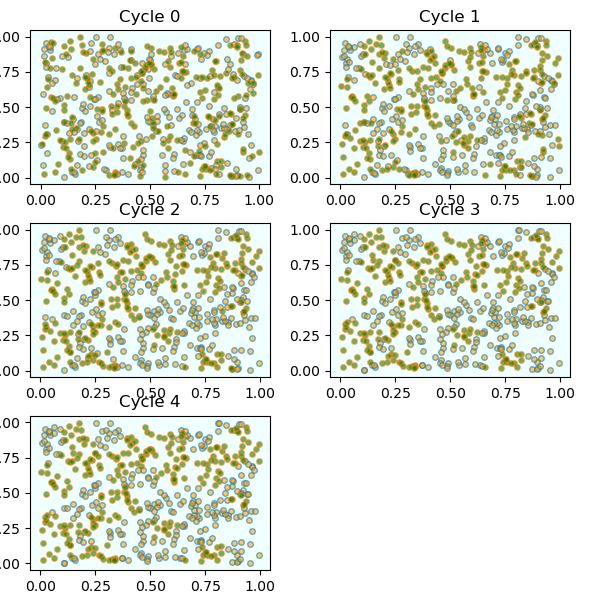
\includegraphics[width=\textwidth]{../../bld/figures/schelling_baseline}

\end{figure}


\begin{figure}
    \caption{Segregation by cycle in the baseline \citet{Schelling69} model, limiting the number of potential moves per period to two}

    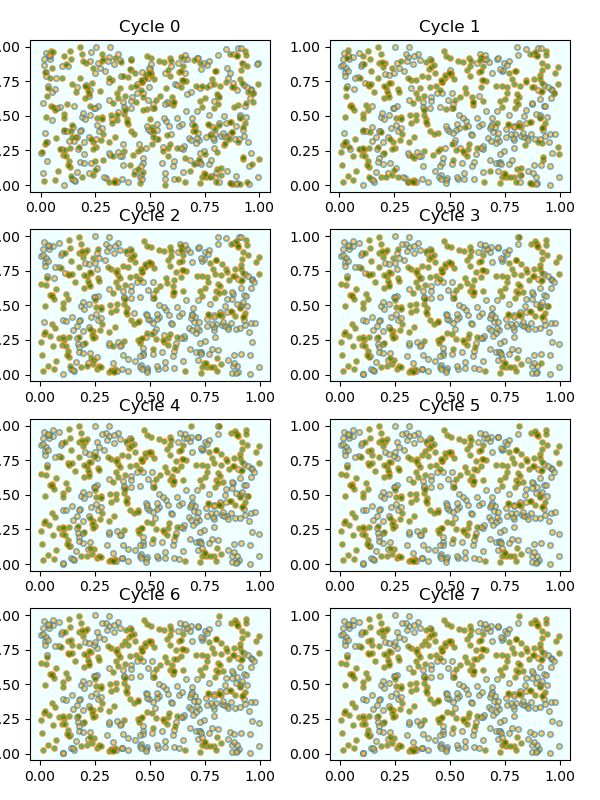
\includegraphics[width=\textwidth]{../../bld/figures/schelling_max_moves_2}

\end{figure}

% section introduction (end)




\setstretch{1}
\printbibliography
\setstretch{1.5}




% \appendix

% The chngctr package is needed for the following lines.
% \counterwithin{table}{section}
% \counterwithin{figure}{section}

\end{document}
